%! TEX program = lualatex
\documentclass[12pt]{scrartcl}
% Packages
%\usepackage[margin=1.5in]{geometry}
\usepackage{index}
\usepackage{amsbsy} % Bold math symbols
\makeindex
%\usepackage[utf8]{inputenc}
\usepackage[T1]{fontenc}
\usepackage{tcolorbox}
\tcbuselibrary{theorems}
\tcbuselibrary{skins}
\tcbuselibrary{breakable}
\usepackage{varwidth}
\usepackage{textcomp}
\usepackage{amsmath, amssymb}
\usepackage{esint}
\usepackage{titlesec}
\usepackage{xcolor}
\usepackage{titling}
\usepackage[linktocpage]{hyperref}
\usepackage{pgfplots}
\usepackage{multicol}
\setlength{\columnsep}{2em}
\usepackage{caption}
\usepackage{amsthm}
\usepackage{import}
\usepackage{cancel}
\usepackage{caption}
\usepackage{nicematrix}
\usepackage{mathrsfs}
\usepackage{mathtools}
%\usepackage{parskip}
\usepackage{enumerate}
\usepackage{graphicx}
\usepackage[italian]{babel}
\usepackage{setspace}
\setstretch{1.2}
% To reset footnote numbering each page
\usepackage[perpage]{footmisc}
\usepackage{faktor}
\usepackage{tikz-cd}
\definecolor{mastercolor}{HTML}{854442}
\definecolor{nred}{HTML}{bf0040}

\usepackage{fancyhdr}
\pagestyle{fancy}

% Titles 
\title{Appunti di\\ \vspace{.3cm} Sistemi dinamici}
\author{Manuel Deodato}
\date{}




\newtheoremstyle{style}% name of the style to be used
{5pt}% measure of space to leave above the theorem. E.g.: 3pt
{5pt}% measure of space to leave below the theorem. E.g.: 3pt
{\normalfont}% name of font to use in the body of the theorem
%{15pt}% measure of space to indent
{0pt}% measure of space to indent
{\noindent\sffamily\scshape\bfseries}% name of head font
{}% punctuation between head and body
{ }% space after theorem head; " " = normal interword space
{\thmname{#1}\thmnumber{ #2}{\thmnote{ (#3)}.\ }}


\theoremstyle{style}
\newtheorem{esempio}{Esempio}[section]
\newtheorem{definizione}{Definizione}[section]
\newtheorem{prop}{Proposizione}[section]
\newtheorem{teorema}{Teorema}[section]
\newtheorem{lemma}{Lemma}[teorema]
\newtheorem{corollario}{Corollario}[teorema]
\newtheorem{osservazione}{Osservazione}[section]
\newtheorem{notazione}{Notazione}[section]
\newtheorem{esercizio}{Esercizio}[section]





\tcolorboxenvironment{definizione}{blanker,breakable,left=5mm,before skip=10pt,after skip=10pt, borderline west={.5mm}{0pt}{mastercolor}, before upper={\setlength{\parindent}{15pt}}}
\tcolorboxenvironment{lemma}{blanker,breakable,left=5mm,before skip=10pt,after skip=10pt, borderline west={.5mm}{0pt}{mastercolor}, before upper={\setlength{\parindent}{15pt}}}
\tcolorboxenvironment{teorema}{enhanced,blanker,breakable,left=5mm,before skip=10pt,after skip=10pt, borderline west={.5mm}{0pt}{mastercolor}, before upper={\setlength{\parindent}{15pt}}}
\tcolorboxenvironment{corollario}{blanker,breakable,left=5mm,before skip=10pt,after skip=10pt, borderline west={.5mm}{0pt}{mastercolor}, before upper={\setlength{\parindent}{15pt}}}
\tcolorboxenvironment{prop}{blanker,breakable,left=5mm,before skip=10pt,after skip=10pt, borderline west={.5mm}{0pt}{mastercolor}, before upper={\setlength{\parindent}{15pt}}}
\tcolorboxenvironment{esempio}{blanker,breakable,left=5mm,before skip=10pt,after skip=10pt, borderline west={.5mm}{0pt}{mastercolor}, before upper={\setlength{\parindent}{15pt}}}
\tcolorboxenvironment{esercizio}{blanker,breakable,left=5mm,before skip=10pt,after skip=10pt, borderline west={.5mm}{0pt}{mastercolor}, before upper={\setlength{\parindent}{15pt}}}
\tcolorboxenvironment{osservazione}{blanker,breakable,left=5mm,before skip=10pt,after skip=10pt, borderline west={.5mm}{0pt}{mastercolor}, before upper={\setlength{\parindent}{15pt}}}


\newenvironment{svolgimento}{\renewcommand\qedsymbol{$\blacksquare$}\begin{proof}[Svolgimento]}{\end{proof}}




%% Generic box
\newtcolorbox{eqbox}[1][]
{
colback=gray!10,
arc=0pt,
boxrule=0pt,
title=#1
}

 \newenvironment{boxenv}[1][]{
    \begin{eqbox}[#1]
    }{
   \end{eqbox}
}



%Captions
\captionsetup[figure]{font=footnotesize,labelfont=footnotesize}
\captionsetup[table]{font=footnotesize,labelfont=footnotesize}
%Titlesec
\titleformat{\section}
{\fontsize{20}{20}\scshape}
{\color{gray}{\fontsize{70}{20}\selectfont\thesection\hspace{.2cm}\color{gray}{\vrule width 1pt}}}
{0.7em}
{}
\titlespacing*{\section}{0pt}{*2}{1cm}
\titlespacing*{\subsection}{0pt}{*5}{.5cm}
\titlespacing*{\subsubsection}{0pt}{*5}{.5cm}

\hypersetup{colorlinks,breaklinks, linkcolor=[RGB]{133,68,66}}

% Personalizza la formattazione della subsection
\titleformat{\subsection}[block]{\centering\fontsize{15}{20}\bfseries}{\color{nred}\normalfont\S\thesubsection}{.5em}{}


% Personalizza la formattazione della subsubsection
\titleformat{\subsubsection}[block]{\centering\fontsize{14}{20}\bfseries}{\color{nred}\normalfont\S\thesubsubsection}{.5em}{}

% Maketitle customization
\renewcommand{\maketitle}{
\begin{center}
{\sffamily
{\fontsize{20}{20}\selectfont\MakeUppercase\thetitle}}

\vspace{0.2in}

{\large\scshape\theauthor}
\end{center}
}

%Evaluate symbol
\DeclareMathOperator{\di}{d\!}
\newcommand*\Eval[3]{\left.#1\right\rvert_{#2}^{#3}}

%%%%%%% Numero delle equazioni in formato a.b
\numberwithin{equation}{subsection}
%%%%%

%%%%%%%%%% Personalizzazione numeri lista
\renewcommand{\theenumi}{(\arabic{enumi})}

%%%% Table of contents

\usepackage[titles]{tocloft}

\renewcommand{\cftdot}{}
\usepackage{titletoc}
%\setcounter{tocdepth}{2}

%%%%%%%%%%%%%%%% Toc style

% Personalizzazione scritta indice


% Font
\renewcommand{\textbf}[1]{\textsf{\bfseries #1}}
\usepackage[osf]{newpxtext}
\usepackage[euler-digits,euler-hat-accent]{eulervm}
%\usepackage{fontspec}
%\DeclareSymbolFont{operators}{OT1}{EBGaramond-TLF}{m}{n}

%%% Hook
\newcommand{\longhookrightarrow}{\lhook\joinrel\longrightarrow}


\begin{document}
\pagestyle{plain}
\maketitle
\vspace{6cm}
\begin{figure}[h!]
	\centering
	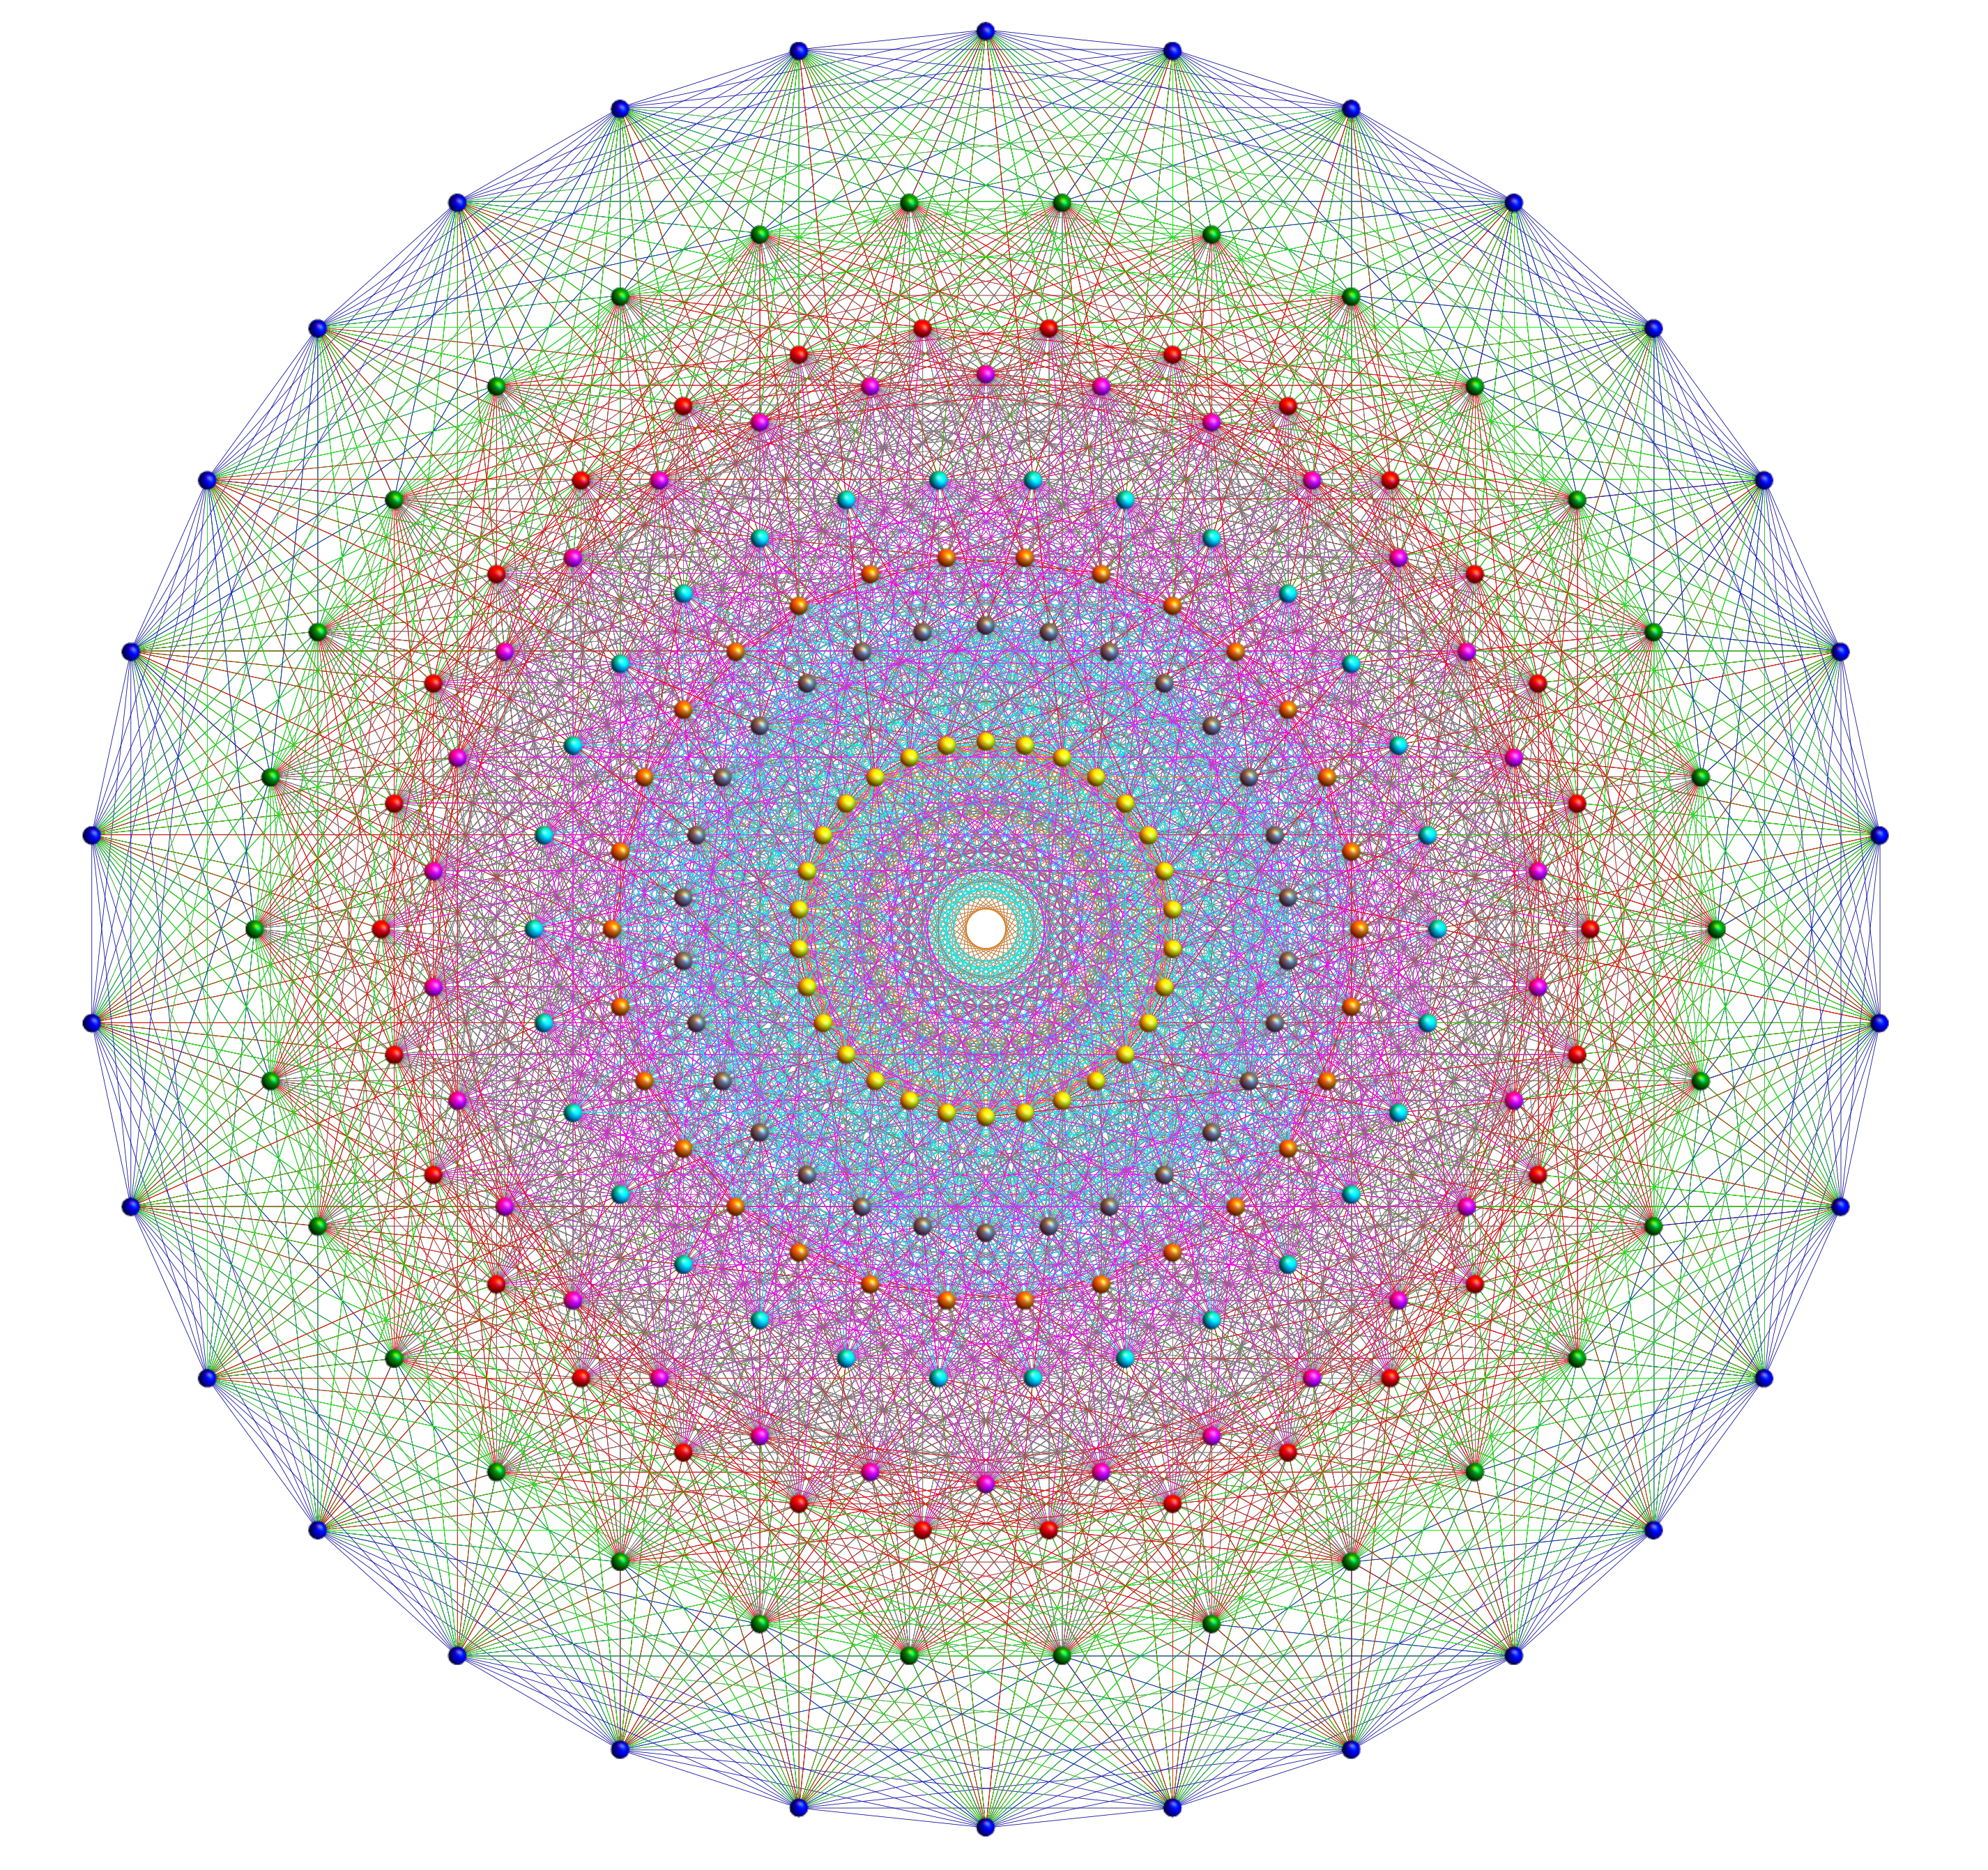
\includegraphics[width=.6\columnwidth]{front.jpeg}
\end{figure}

\newpage
\pagestyle{plain}
\tableofcontents 
\newpage
\pagestyle{fancy}
\section{Equazioni differenziali ordinarie}
\subsection{Introduzione}

\begin{definizione}
	[Equazione differenziale]
	Un'equazione differenziale ordinaria di ordine $k$ \`e un'equazione della forma
	\[
	F\big(x,y(x),\ldots, y^{(k)} (x)\big) = 0 
	\] 
	con $F : I \times (\mathbb{R}^n)^k \to \mathbb{R}$ continua e $I \subseteq \mathbb{R}$.
	La funzione $y : I \to \mathbb{R}^n$ \`e detta \textit{funzione incognita}.
\end{definizione}
\noindent In alcuni casi, \`e possibile riscrivere l'equazione differenziale esplicitando in un membro il termine il cui ordine di derivazione \`e massimo, ossia si pu\`o scrivere
\[
y^{(k)} (x) = \widetilde{F}\big(x ,y(x) ,\ldots,y^{(k-1)} (x)\big)
\] 
In questo caso, si dice che l'equazione \`e in \textit{forma esplicita}.
\begin{osservazione}
Tramite il cambio di variabili
\[
Y(x) = \begin{pmatrix} y(x)\\ \vdots\\ y^{(k-1)} (x) \end{pmatrix} \in \mathbb{R}^{nk} 
\] 
\`e possibile riscrivere un'equazione differenziale di ordine $k$ nella forma $Y'= f(x,Y)$, con 
\[
f(x,Y) = \begin{pmatrix} y'(x)\\ y''(x) \\ \vdots\\ F(x,y,\ldots,y^{(k-1)}) \end{pmatrix} \in \mathbb{R}^{nk} 
\] 
Questo significa che, indipendentemente dall'ordine dell'equazione di partenza, fin tanto che questa \`e esprimibile in forma esplicita, \`e sempre possibile ricondursi a un sistema di equazioni del primo ordine.
Nel caso in cui l'equazione non fosse esprimibile in forma esplicita, \`e necessario ricorrere al teorema della funzione implicita; se questo non fosse applicabile, allora il ragionamento non sarebbe valido.
\end{osservazione}
\noindent Quest'ultima osservazione permette di sviluppare la teoria delle equazioni differenziali per equazioni del primo ordine.

\begin{definizione}
	[Problema di Cauchy]
	Sia data un'equazione differenziale $y' = f(x,y)$, con $f : I \times A \to \mathbb{R}^n$ e $A \subseteq \mathbb{R}^n$ aperto; un sistema del tipo
	\[
	\begin{cases}
		y' = f(x,y)\\
		y(x_0) = y_0
	\end{cases}
	\] 
	con $(x_0,y_0) \in I \times A$ \`e detto \textit{problema di Cauchy}, mentre il valore $y_0$ \`e detto \textit{dato iniziale}.
\end{definizione}
\noindent La soluzione di un problema di Cauchy della forma
\[
\begin{cases}
	y' = f(x,y)\\
	y(x_0) = y_0
\end{cases}
\] 
\`e esprimibile in forma integrale come
\begin{equation}
	y(x) = y_0 + \int_{x_0} ^x f(t,y(t)) \ dt
\end{equation}
Infatti, una funzione $y(x)$ risolve il problema di Cauchy se e solo se risolve l'equazione integrale.
Ne segue, inoltre, che ogni funzione $y$ che soddisfa il problema di Cauchy, vista la forma integrale appena trovata, deve essere di classe $C^1$.
\begin{boxenv}[]
Per il resto della trattazione, si assumer\`a che l'equazione differenziale in esame sia della forma
\[
y'=f(x,y)
\] 
e che i problemi di Cauchy trattati siano della forma
\[
\begin{cases}
	y'  = f(x,y)\\
	y(x_0) = y_0
\end{cases}
\] 
Inoltre, si assumer\`a sempre che $A = B_r(y_0)$ e si user\`a la notazione
\[
I_a = (x_0-a,x_0+a)
\] 
\end{boxenv}
\begin{definizione}
		[Funzione uniformemente lipschitziana]
		Una funzione $f(x,y) : I_a \times B_r(y_0)\to \mathbb{R}^n$ \`e detta \textit{uniformemente $L$-lipschitziana} in $y$ se $\exists L>0$ tale che $\forall (x,y_1), (x,y_2) \in I_a \times B_r(y_0)$ \`e soddisfatta la relazione
		\[
		\lvert f(x,y_1) - f(x,y_2) \rvert \le L\lvert y_1-y_2 \rvert 
		\] 
\end{definizione}
\begin{teorema}
	[Teorema di Cauchy-Lipschitz]
	Sia $f : I_a \times B_r(y_0)\to \mathbb{R}^n$ una funzione continua, limitata e uniformemente $L$-lipschitziana nelle $y$; allora $\exists \delta \in (0,a]$ e $\exists ! y \in C^1(I_\delta ,\mathbb{R}^n)$ soluzione del problema di Cauchy con dato iniziale $(x_0,y_0)$.
	\begin{proof}
		Sia $\delta >0$ e sia $X = \big(C(I_\delta ,\mathbb{R}^n),\left\lVert \cdot  \right\rVert _\infty\big)$, con $I_\delta = [x_0-\delta ,x_0+\delta ]$.
		Sia, inoltre
		\[
		X_{\delta ,r} = \left\{ y \in C(I_\delta ,\mathbb{R}^n) \mid y(x) \in \overline{B_r}(y_0), \ \forall x \in I_\delta  \right\} 
		\] 
		che \`e chiuso in $C(I_\delta ,\mathbb{R}^n)$; in particolare, $X_{\delta ,r} $ \`e uno spazio metrico completo.
	\end{proof}
\end{teorema}






\end{document}
